% Algorithm XXX: MQSI---Monotone quintic spline interpolation,
% Thomas C.H. Lux, Layne T. Watson, Tyler H. Chang,
% William Thacker, Kirk W. Cameron, and Yili Hong
% ACM Trans. Math. Software, ?/?/2020.
% 
%
\magnification=1000 \hsize=30pc \vsize=47pc
\parindent=10pt \parskip=0pt plus 3pt
\baselineskip=13pt plus 2pt minus 1pt \lineskiplimit=2pt
\lineskip=2pt plus 2pt                                  %\raggedright
\tolerance=800
%\abovedisplayskip=6pt plus 6pt minus 3pt
%\abovedisplayshortskip=0pt plus 3pt
%\belowdisplayskip=6pt plus 6pt minus 3pt
%\belowdisplayshortskip=6pt plus 2pt minus 3pt

% eplain package, mainly for its bibliography management.
\input eplain

% Color definitions.
\input colordvi
\def\BEGINC{\textPeach} \def\ENDC{\textBlack}
\def\red#1{\BEGINC#1\ENDC}
\let\beginred=\BEGINC
\let\endred=\ENDC

% Commands for inserting an 'algorithm' section.
\def\indented#1{{\leftskip=1cm}{#1}{\leftskip=0cm}}
\def\comment#1{\vskip 10mm {\it #1} \vskip 10mm}%
\def\thickrule{\hrule\hrule\hrule}

% fonts
\font\itVIII=cmti8 \font\slVIII=cmsl8 \font\bfVIII=cmbx8
\font\ttVIII=cmtt8 \font\caps=cmcsc10 \font\capsVIII=cmcsc10 at 8pt
\font\ttXVIII=cmtt12 at 18pt \font\eightmi=cmmi8 \font\eightsy=cmsy8
\font\rmeight=cmr8  \def\rmVIII{\rmeight \baselineskip=10pt plus 2pt
minus 1pt \lineskiplimit=2pt \lineskip=2pt plus 1pt
\parskip=0pt \textfont0=\rmeight \textfont1=\eightmi \textfont2=\eightsy}
\font\hlvXVIII=phvr at 18pt \font\hlvVIII=phvr at 8pt \font\hlv=phvr

% math blackboard font
\font\tenamsb=msbm10 \font\sevenamsb=msbm7 \font\fiveamsb=msbm5
\newfam\bbfam
\textfont\bbfam=\tenamsb
\scriptfont\bbfam=\sevenamsb
\scriptscriptfont\bbfam=\fiveamsb
\def\bbb{\fam\bbfam}

\input epsf %Postscript figures.
\def\lcaption#1#2{{\noindent\rmVIII Fig.~#1. #2\par}}
\def\ltabcaption#1#2{{\noindent\rmVIII Table #1. #2\par}}


% other definitions.
\def\h{\par\hangindent=10pt\hangafter=1\noindent}
\def\heading#1{\par\bigskip\leftline{\hlv#1}\nobreak\smallskip
\noindent\ignorespaces}
\newdimen\headdigit{\setbox11=\hbox{\hlv 8. }\global\headdigit=\wd11}
\def\footnoterule{\bigskip\kern-3pt \hrule \kern 2.6pt \smallskip}
\def\bullitem{\par\vskip 2pt plus 2pt\hangindent=15pt \hangafter=1
\noindent\hbox to 15pt{---\hfil}\ignorespaces}
\def\bulllitem{\par\vskip 2pt plus 2pt\hangindent=30pt
\hangafter=1 \noindent\hskip 15pt\hbox to
15pt{---\hfil}\ignorespaces}
\def\Th#1 #2\par{\par\medskip{\it{\caps#1}. #2}\par\medskip}
\def\btable#1{\topinsert \rmVIII \let\bf=\bfVIII \textfont0=\scriptfont0
\scriptfont0=\scriptscriptfont0 \textfont1=\scriptfont1
\scriptfont1=\scriptscriptfont1 \centerline{#1}}
\let\xpar=\par
\def\ds{\displaystyle}\def\ab{\allowbreak}

% math definitions
\def\tn#1{\left\Vert #1\right\Vert_2}
\def\mn#1{\left\Vert #1\right\Vert_\infty}
\def\lee{\mathrel{\vcenter{\hbox{$\scriptstyle\mathord<$}\nointerlineskip
\vskip 1pt\hbox{$\scriptstyle\mathord=$}}}}
\def\gee{\mathrel{\vcenter{\hbox{$\scriptstyle\mathord>$}\nointerlineskip
\vskip 1pt\hbox{$\scriptstyle\mathord=$}}}}
\def\real{\mathop{\rm I\!R}\nolimits}
\def\R{{\bf R}}
\def\Rd{{\bf R}^d}
\def\Rdd{{\bf R}^{d\times d}}
%\def\bull{\hfill \vrule height6pt width6pt depth0pt}
\def\:{\mathrel{:\mathord=}}

% OUTPUT
\def\rightheadline{\hfill\hlvVIII\rightrh\hskip20pt$\scriptstyle\bullet$\hskip
20pt\folio}
\def\leftheadline{\hlvVIII\folio\hskip20pt$\scriptstyle\bullet$\hskip
20pt\leftrh\hfill}
\footline={\hfill}%no page number on first page
\output{\plainoutput}
\def\plainoutput{\shipout\vbox{\makeheadline\pagebody\makefootline}
  \advancepageno \global\footline={\hfill}
  \ifodd\pageno
        \global\headline={\rightheadline}
  \else
        \global\headline={\leftheadline}
  \fi
  \ifnum\outputpenalty>-20000 \else\dosupereject\fi}
\def\pagebody{\vbox to\vsize{\boxmaxdepth\maxdepth \pagecontents}}
\def\makeheadline{\vbox to 0pt{\vskip-22.5pt
  \line{\vbox to8.5pt{}\the\headline}\vss}\nointerlineskip}
\def\makefootline{\baselineskip24pt\vskip-6pt\line{\the\footline}}
\def\dosupereject{\ifnum\insertpenalties>0pt
  \line{}\kern-\topskip\nobreak\vfill\supereject\fi}
%\def\footnoterule{\vskip10pt\kern-3pt \hrule width 3em \kern 2.6pt}

\def\leftrh{Lux et al.}
\def\rightrh{Algorithm XXX: MQSI}

{\baselineskip=24pt \leftline{\hlvXVIII Algorithm XXX: MQSI: Monotone Quintic}
\leftline{\hlvXVIII Spline Interpolation}}
\bigskip\medskip
\leftline{\hlv THOMAS C.H. LUX, LAYNE T. WATSON, TYLER H. CHANG,}
\smallskip
\leftline{\hlv WILLIAM THACKER, KIRK W. CAMERON, AND YILI HONG}
\smallskip
\leftline{\hlv Virginia Polytechnic Institute and State University}
\bigskip

\hrule\bigskip\smallskip \footnote{}{\hskip
-\parindent{\parindent=0pt\rmVIII Authors' addresses:
T. C. H. Lux, T. H. Chang, K. W. Cameron,
Department of Computer Science, L. T. Watson,
Departments of Computer Science, Mathematics, and Aerospace and Ocean
Engineering, Y. Hong, Department of Statistics, Virginia
Polytechnic Institute \& State University, Blacksburg, VA 24061;
e-mail: {\ttVIII tchlux@vt.edu}. \xpar
% Permission to make digital/hard copy of
%part or all of this work for personal or classroom use is granted
%without fee provided that the copies are not made or distributed for
%profit or commercial advantage, the copyright notice, the title of
%the publication, and its date appear, and notice is given that
%copying is by permission of the ACM, Inc. To copy otherwise, to
%republish, to post on servers, or to redistribute to lists, requires
%specific permission and/or fee. \xpar\copyright\ 2018 by the
%Association for Computing Machinery, Inc. \xpar 
}}

% Abstract and Introduction
{\rmVIII\parindent=0pt MQSI contains a serial code written in Fortran
  1995 for constructing monotone quintic spline interpolants to
  data. Using sharp theoretical monotonicity constraints, first and
  second derivative estimates at data provided by a quadratic facet
  model are refined to produce a $C^2$ monotone interpolant. This
  paper includes algorithm and implementation details, complexity and
  sensitivity analyses, usage information, and a brief performance
  study.

\medskip
Categories and Subject Descriptors: G.1.1 [{\bfVIII Numerical Analysis}]:
Interpolation --- Spline and piecewise polynomial interpolation;
J.2 [{\bfVIII Computer Applications}]: Physical Science and Engineering
--- {\itVIII Mathematics};
G.4 [{\bfVIII Mathematics of Computing}]: Mathematical Software

\medskip
General Terms: Algorithms, Monotonicity, Documentation

\medskip
Additional Key Words and Phrases: Quintic Spline, interpolation

}

\bigskip\hrule\bigskip\medskip
\heading{1. INTRODUCTION}


Many domains of science rely on smooth approximations to real-valued
functions over a closed interval. Piecewise polynomial functions
(splines) provide the smooth approximations for animation in graphics
\cite{herman2015techniques,quint2003scalable}, aesthetic structural
support in architecture \cite{brennan2019measure}, efficient
aerodynamic surfaces in automotive and aerospace engineering
\cite{brennan2019measure}, prolonged effective operation of electric
motors \cite{berglund2009planning}, and accurate nonparametric
approximations in statistics \cite{knott2012interpolating}. While
polynomial interpolants and regressors apply broadly, splines are
often a good choice because they can approximate globally complex
functions while minimizing the local complexity of an approximation.

It is often the case that the true underlying function or phenomenon
being modeled has known properties e.g., convexity, positivity,
various levels of continuity, or monotonicity. Given a reasonable
amount of data, it quickly becomes difficult to achieve desirable
properties in a single polynomial function. In general, the
maintenance of function properties through interpolation/regression is
referred to as {\it shape preserving}
\cite{fritsch1980monotone,gregory1985shape}. The specific shapes this
work will achieve in approximations are monotonicity and $C^2$
continuity. These properties are chiefly important to the
approximation of cumulative distribution functions and subsequently
the effective generation of random numbers from a specified
distribution.

In statistics especially, the construction of a monotone interpolating
spline that is $C^2$ continuous is meaningfully useful
\cite{ramsay1988monotone}. A function with these properties could
approximate a cumulative distribution function to a high level of
accuracy with relatively few intervals. A twice continuously
differentiable approximation to a cumulative distribution function
(CDF) would also produce a corresponding probability density function
(PDF) that is continuously differentiable, which is a property many
standard parametric distributions maintain.

The currently available software for monotone piecewise polynomial
interpolation includes quadratic \cite{he1998monotone}, cubic
\cite{fritsch1980monotone}, and (with limited application) quartic
\cite{wang2004rational,piah2011improved,yao2018unconditionally}
cases. In addition, a statistical method for bootstrapping the
construction of an arbitrarily smooth monotone fit exists
\cite{leitenstorfer2006generalized}, but the method does not take
advantage of known analytic properties related to quintic
polynomials. Theory has been provided for the quintic case
\cite{ulrich1994positivity,hess1994positive}, however this theory has
not yet been used to construct a monotone quintic spline interpolation
routine. Recent work suggests that the lack of quintic software may be
due to a general unawareness of the theory
\cite{xie2018semiparametric}.


\topinsert
\centerline{\epsfxsize=4.5truein \epsffile{vt_logo.eps}}
{\narrower\noindent\rmVIII Fig.\ 1.
Example polynomials that interpolate function values at the ends of
the interval $[0,1]$. The first only interpolates the function values
$g_2(0) = 1$ and $g_2(1) = 0$, making it the order two polynomial
$g_2(x) = 1 - x$. For the second plot $g_4(x) = 8x^3 - 12x^2 + 4x +
1/2$, which is order four and interpolates the values $g_4(0) = 1/2$,
$g_4'(0) = 4$, $g_4(1) = 1/2$, $g_4'(1) = 4$. Finally the third plot
shows the order six polynomial $g_6(x) = - 64x^5 + 160x^4 - 140x^3 +
50x^2 - 7x + 1$ interpolating the function values $g_6(0) = 1$,
$g_6'(0) = -7$, $g_6''(0) = 100$, $g_6(1) = 0$, $g_6'(1) = -7$,
$g_6''(1) = -100$. Notice that interpolating the same fixed number of
function values at each endpoint will always result in an even order
interpolating polynomial.
\par}
\endinsert

The importance of piecewise quintic interpolation over lower order
approximations can be simply demonstrated. In general, the order of a
polynomial determines the number of function values it can
interpolate, and the growth rate of error away from the interpolated
function values. As demonstrated in Figure
\ref{fig:spline_demonstration}, it can be seen that matching a value
at either end of the interval requires an order two (linear)
approximation and each additional derivative at the ends of the
interval raises the necessary polynomial order by two. Hence, only
even order (odd degree) interpolating splines are broadly
applicable. The body of this work is composed of a novel algorithm for
enforcing monotonicity on quintic polynomial pieces, then extending
that solution to work on quintic splines.

The major contribution of this work is an algorithm for constructing
monotone quintic interpolating splines that utilizes existing quintic
monotonicity theory. The remainder of this paper is structured as
follows: Section \ref{sec:monotone-cubic} summarizes the existing
monotone cubic spline interpolation methodology, Section
\ref{sec:monotone-quintic} presents an algorithm for constructing
monotone quintic spline interpolants, Section \ref{sec:results} offers
experiments and results with cubic and quintic methods, Sections
\ref{sec:discussion} and \ref{sec:conclusion} discuss results and
conclude.



\heading{1.1 \enspace Computing a Monotone Cubic Interpolant}

The current state-of-the-art monotone interpolating spline with a
mathematical software implementation is piecewise cubic, continuously
differentiable, and was first proposed in \cite{fritsch1980monotone}
then expanded upon in \cite{carlson1985monotone}. Let $\pi: x_0 = k_1
< k_2 < \cdots < k_n = x_1$ be a partition of the interval
$[x_0,x_1]$. Let $f: {\bbb R} \rightarrow {\bbb R}$ be $C^2$, and
$\bigl\{f(k_i)\bigr\}_{i=1}^n$ and $\bigl\{\Delta_i\bigr\}_{i=1}^n$ be
given sets of function and derivative values at the partition points
for a monotone function $f$. Either $f(k_i) \leq f(k_{i+1})$, $i=1$,
$\ldots$, $n-1$, and $\Delta_i\ge0$, $i=1$, $\ldots$, $n$, or $f(k_i)
\geq f(k_{i+1})$, $i=1$, $\ldots$, $n-1$, and $\Delta_i\le0$, $i=1$,
$\ldots$, $n$. Let $\hat f$ be a piecewise cubic polynomial defined in
each subinterval $I_i = [k_i, k_{i+1}]$ by
$$ h_i = k_{i+1} - k_{i}, \quad u(t) = 3t^2 - 2t^3, \quad p(t) = t^3 - t^2,$$
$$\hat f(x) = f(k_i) u\big((k_{i+1} - x) / h_i\big) + f(k_{i+1}) u\big((x - k_i) / h_i\big) $$
$$ - h_i\Delta_i p\big((k_{i+1}-x)/h_i\big) + h_i\Delta_{i+1} p\big((x-k_i)/h_i\big).$$ 
Notice that a trivially monotone spline results when $\Delta_i = 0$,
for $i = 1$, $\ldots$, $n$. However, such a spline has too many
{\it wiggles} for most applications. \cite{carlson1985monotone}
show that simple conditions on the derivative values can guarantee
monotonicity, and that these conditions can be enforced in a way that
ensures modifications on one interval will not break the monotonicity
of cubic polynomials over any neighboring intervals. If $f(k_i) =
f(k_{i+1})$, take $\Delta_i = \Delta_{i+1} =0$ and $\alpha =\beta =1$,
otherwise let $\alpha = \big(\Delta_i (k_{i+1}-k_i)\big) /
\big(f(k_{i+1}) - f(k_i)\big)$ and $\beta =
\big(\Delta_{i+1}(k_{i+1}-k_i)\big) / \big(f(k_{i+1}) -
f(k_i)\big)$. Monotonicity of a cubic polynomial over a subinterval
can be maintained by ensuring that $\alpha$ and $\beta$ reside in any
of the regions depicted in Figure \ref{fig:projection}.

\topinsert
\centerline{\epsfxsize=4.5truein \epsffile{vt_logo.eps}}
{\narrower\noindent\rmVIII Fig.\ 2.
These are the feasible regions of monotonicity for cubic splines and
the projections that make a cubic polynomial piece monotone. The
regions themselves are numbered 1--4 corresponding to their original
description in Fritsch and Carlson (1980). One point is projected onto
each region as a demonstration.
\par}
\endinsert

The actual region of monotonicity for a cubic polynomial is larger,
but projection of $(\alpha, \beta)$ into one of these regions ensures
that monotonicity will be achieved and not violated for neighboring
regions. The user must decide which region is most appropriate for the
projections based on the application, Fritsch and Carlson recommend
using Region 2.

While the cubic monotonicity case affords such a concise solution, the
region of monotonicity is not so simple in the quintic case. In the
next section, an algorithm for performing a projection similar to
those for cubic polynomials is proposed.

\heading{2. MONOTONE QUINTIC INTERPOLATION}

The following section is composed of three algorithms that together
are used to construct a monotone quintic spline interpolant. Without
loss of generality, the algorithms will only consider the monotone
increasing (nondecreasing) case. The monotone decreasing case is
handled similarly. Algorithm \ref{alg:check-monotone} checks
monotonicity, Algorithm \ref{alg:make-monotone} enforces monotonicity
on an order six polynomial piece of the quintic spline, and Algorithm
\ref{alg:monotone-spline} uses the previous two algorithms to enforce
monotonicity for the entire quintic spline.


In pseudocode, a function {\tt binary\_search($g,$ $a,$ $b$)} is
used, where $a,b\in S\subset {\bbb R}^p$ for convex $S$, $g: S
\rightarrow \{${\tt FALSE}, {\tt TRUE}$\}$ is a right continuous
Boolean function, $g(b) = \hbox{{\tt TRUE}}$, and for $\mu \in
[0,1]$, $g\big((1-\mu)a + \mu b\big) =\hbox{{\tt TRUE}}
\Longrightarrow g\big((1-\nu)a + \nu b\big) =\hbox{{\tt TRUE}}$ for
$\mu \le \nu\le1$. The search returns $\big((1-c)a + c b\big)$ for the
smallest $c \in [0,1]$ such that $g\big((1-c)a + c b\big) =
\hbox{{\tt TRUE}}$.

These algorithms make use of first and second derivatives of the approximated function where $D$ denotes the differentiation operator. In the case that the first and second derivative information is not provided along with function values, the derivatives are estimated with finite differences of the function values. The final quintic spline is represented as a piecewise polynomial using the Newton form for each polynomial piece, and ultimately converted to a $B$-spline representation for evaluation.

\def\newline{\hfil\break}

\parindent=0pt
\vskip 5mm
\thickrule
{\bf Algorithm 1:} {\tt is\_monotone}$\big(x_0, x_1, f \big)$ \newline
where $x_0$, $x_1 \in {\bbb R}$, $x_0 < x_1$, and $f$ is an order six
polynomial defined by $f(x_0)$, $Df(x_0)$, $D^2f(x_0)$, $f(x_1)$,
$Df(x_1)$, $D^2f(x_1)$. Returns {\tt TRUE} if $f$ is monotone
increasing on $[x_0,x_1]$.
\hrule
\vskip 3mm
\numberedlist
{\tt
\li if $\big(f(x_0) = f(x_1)\big)$ and not $\big( 0 = Df(x_0) = Df(x_1) = D^2f(x_0) = D^2f(x_1) \big)$
\li \indented{return FALSE} \newline
end if \newline
\li if $\big(Df(x_0) < 0$ or $Df(x_1) < 0\big)$ \newline
    \indented{return FALSE} \newline
    end if \newline
    \comment{The necessity of these first two steps follows directly from the fact that $f$ is $C^2$. The next case is in accordance with a simplified condition for quintic monotonicity that reduces to one of cubic positivity studied in \cite{schmidt1988positivity}, where $\alpha$, $\beta$, $\gamma$, and $\delta$ are defined in terms of values and derivatives of $f$ at $x_0$ and $x_1$. Step \ref{alg1-alpha} checks for the necessary condition that $\alpha \ge 0$, Step \ref{alg1-beta} checks $\beta \geq \alpha$, and Step \ref{alg1-gamma} checks $\gamma \geq \delta$, all from \cite{schmidt1988positivity}. If all necessary conditions are met, then the order six piece is monotone and Step \ref{alg1-simplified-true} concludes this check.}
  if $\big(Df(x_0) = 0$ or $Df(x_1) = 0\big)$ \newline
  \indented{$w := x_0 - x_1$} \newline
  \indented{$v := f(x_0) - f(x_1)$} \newline
  \indented{if $\big(D^2f(x_1) > {-4}Df(x_1) / w \big)$ return FALSE} \newline
  \indented{if $\big(D^2f(x_1) < (3w D^2f(x_0) - 24 Df(x_0) - 32
    Df(x_1) + 60v/w) / (5w) \big)$ return FALSE} \newline
  \indented{if $\big(D^2f(x_0) < 3 Df(x_0) / w \big)$ return FALSE} \newline
  \indented{return TRUE} \newline
    end if \newline
    \comment{The following code considers the remaining case where $Df(x_0) \neq 0$ and $Df(x_1) \neq 0$.} \newline
  $\displaystyle A := Df(x_0){x_1 - x_0 \over f(x_1) - f(x_0)}$ \newline
  $\displaystyle B := Df(x_1) {x_1 - x_0 \over f(x_1) - f(x_0)}$ \newline
    \comment{The variables $A$ and $B$ correspond directly to the theoretical foundation for positive quartic polynomials established in \cite{ulrich1994positivity}, first defined after Equation (18).} \newline
  $\displaystyle \gamma_0 := 4 {Df(x_0) \over Df(x_1)} (B/A)^{3/4}$ \newline
  $\displaystyle \gamma_1 := {x_1 - x_0 \over Df(x_1)} (B/A)^{3/4}$ \newline
  $\alpha_0 := 4 (B/A)^{1/4}$ \newline
  $\displaystyle \alpha_1 := -{x_1 - x_0 \over Df(x_1)} (B/A)^{1/4}$ \newline 
  $\displaystyle \beta_0 := 30 - {12 \big(Df(x_0) + Df(x_1)\big) (x_1 - x_0) \over \big(f(x_1) - f(x_0)\big) \sqrt{A}\sqrt{B}}$ \newline
  $\displaystyle \beta_1 := {-3 (x_1 - x_0)^2 \over 2 \big(f(x_1) - f(x_0)\big) \sqrt{A} \sqrt{B}} $ \newline
    \comment{The $\gamma$, $\alpha$, and $\beta$ terms with subscripts $0$ and $1$ are algebraic reductions of the simplified conditions for satisfying Theorem 2 in Equation (16) of \cite{ulrich1994positivity}. These terms with subscripts $0$ and $1$ make the computation of $\alpha$, $\beta$, and $\gamma$ functions of the second derivative terms, as seen in Step \ref{alg1-abg} below.} \newline
  $\gamma := \gamma_0 + \gamma_1 D^2f(x_0)$ \newline
  $\alpha := \alpha_0 + \alpha_1 D^2f(x_1)$ \newline
  $\beta := \beta_0 + \beta_1 \big(D^2f(x_0) - D^2f(x_1)\big)$ \newline
  if $(\beta \leq 6)$ return $\big(\alpha > - (\beta + 2) / 2\big)$ \newline
  else $\qquad$ return $\big(\gamma > -2 \sqrt{\beta - 2}\big)$ \newline
  end if \newline
}
\endnumberedlist
\vskip 2mm
\hrule
\vskip 3mm
\parindent=10pt

%% ----------------------------------------------------------------------

The reason for structuring the $\alpha$, $\beta$, and $\gamma$ computations in terms of the second derivative of $f$ (seen in Step \ref{alg1-abg} of Algorithm \ref{alg:check-monotone}) will become more apparent later. The next problem to consider is that of making a nonmonotone order six polynomial piece into a monotone one by modifying its first and second derivative values at the ends of an interval. Note that the actual value of the function at the ends of the interval is not modified, as the resulting polynomial needs to interpolate.


Notice that both Algorithms \ref{alg:check-monotone} and \ref{alg:make-monotone} have ${\cal O}(1)$ runtime assuming a fixed level of precision is chosen beforehand. A constant number of operations are needed for verifying monotonicity (Algorithm \ref{alg:check-monotone}), while a constant set of operations and a single binary search are performed for enforcing monotonicity (Algorithm \ref{alg:make-monotone}). The search requires a fixed number of steps to achieve any predetermined relative precision, since its accuracy is predetermined and not a function of the problem at hand. Also note that an efficient implementation of Algorithm \ref{alg:make-monotone} only needs to recalculate Steps \ref{alg1-abg} and \ref{alg1-last} of Algorithm \ref{alg:check-monotone} during the binary search. Next, an algorithm for constructing a monotone quintic spline interpolant is presented.

%% ----------------------------------------------------------------------

\vskip 5mm
\thickrule
{\bf Algorithm 2:} {\tt monotone\_spline}$\big((k_1$, $\ldots$, $k_n)$, $f$, $s\big)$
where $(k_1$, $\ldots$, $k_n)$ is an increasing sequence of real
numbers, $f$ is an order six piecewise polynomial with breakpoints
$k_1$, $\ldots$, $k_n$ defined by the data
$\bigl\{f(k_i)\bigr\}_{i=1}^n$, $\bigl\{Df(k_i)\bigr\}_{i=1}^n$,
$\bigl\{D^2f(k_i)\bigr\}_{i=1}^n$, and $s > 1$ is an integer shrink
factor.
\hrule
\vskip 3mm
    \newline create queue
      \newline create changed$(1$, $\ldots$, $n) := $ FALSE
      \newline create step\_size$(1$, $\ldots$, $n) := \bigl(Df(k_1)/s$, $\ldots$, $Df(k_n)/s\bigr)$
      \comment{The three variables defined in Step \ref{step:create} are used to ensure the eventual achievement of monotonicity. The {\tt queue} is a standard first in first out (FIFO) queue with {\tt enqueue} and {\tt dequeue} operations. The array {\tt changed} contains Booleans describing whether or not a breakpoint belongs to an interval that has been modified to enforce monotonicity. The {\tt step\_size} array contains the real-valued derivative decrement step sizes to use in the search for a valid monotone spline.}
    \newline for $i := 1$, $\ldots$, $n-1$
      \indented{enqueue $\bigl((k_i, k_{i+1})\bigr)$}
      end for
      \comment{Initially, all intervals must be checked for monotonicity. The following loop will continue until all intervals are verified as monotone without need for modification.}
    \newline while $($size$($queue$) > 0)$
    \newline \indented{$(k_j$, $k_{j+1}) := $ dequeue}
    \newline \indented{if $\big($not is\_monotone$(k_j$, $k_{j+1}$, $f)\big)$}
    \newline \indented{\indented{if $\big($changed$(j)\big) \qquad \ Df(k_j) := Df(k_j) -{}$step\_size$(j)$}}
      \indented{\indented{if $\big($changed$(j+1)\big) \quad Df(k_{j+1}) := Df(k_{j+1}) -{}$step\_size$(j+1)$}}
      \indented{\indented{\comment{If a breakpoint belongs to an interval that has been previously modified, then the enforced monotonicity conditions on the second derivatives of adjacent intervals must contradict one another. In turn, the involved first derivatives are decreased towards zero by a predetermined step size.}}}
    \newline \indented{\indented{make\_monotone$(k_j,\ k_{j+1},\ f)$}}
    \newline \indented{\indented{changed$(j) :=$ TRUE}}
      \indented{\indented{changed$(j+1) :=$ TRUE}}
    \newline \indented{\indented{if $\big(j > 1$ and $(k_{j-1}, k_j) \not\in$ queue$\big)$ enqueue $\bigl((k_{j-1}, k_j)\bigr)$}}
      \indented{\indented{enqueue $\bigl((k_j, k_{j+1})\bigr)$}}
      \indented{\indented{if $\big(j+1 < n$ and $(k_{j+1}, k_{j+2}) \not\in$ queue$\big)$ enqueue $\bigl((k_{j+1}, k_{j+2})\bigr)$}}
      \indented{\indented{\comment{Step \ref{step:changed} records the endpoints of the current interval as having been changed, while \ref{step:requeue} adds adjacent intervals to {\tt queue} that may have inadvertently been made nonmonotone by the changes to the present interval.}}}      
      \indented{end if}
      end while
\vskip 2mm
\hrule
\vskip 3mm

%% ----------------------------------------------------------------------

It is mentioned in \cite{ulrich1994positivity} that for sufficiently small $Df(k_i)$ and $Df(k_{i+1})$ the admissible solution interval of second derivative values becomes arbitrarily large. It can also be seen that decreasing the assigned derivative values towards zero will eventually cause Steps \ref{alg1-alpha} through \ref{alg1-gamma} of Algorithm \ref{alg:check-monotone} to all fail, resulting in Step \ref{alg1-simplified-true} returning {\tt TRUE}.

If successive monotonicity fixes are required for all intervals, the worst case runtime of Algorithm \ref{alg:monotone-spline} is ${\cal O}(s n)$ for $n$ breakpoints and shrink factor $s$. In practice this worst case has been observed to be unlikely.

\heading{3. EXPERIMENTAL RESULTS}

Given the increased order of approximation, it is naturally expected that some accuracy benefit could be gained by using a quintic spline over a cubic spline. Experiments 1 and 2 below test some accuracy differences between monotone cubic and quintic splines. Experiment 3 analyzes the number of operations performed by Algorithm \ref{alg:monotone-spline} with increasingly large samples of monotone data.

\heading{3.1 \enspace Approximating a Trigonometric Function}

For this experiment, the function $\sin(x) + x$ is considered over the interval $[0,(5/2)\pi]$ as seen in Figure \ref{fig:cubic_quintic_sin}. Given an increasing number of points, the maximum error of cubic and quintic approximations is shown in Figure \ref{fig:experiment_1}. The quintic approximation consistently has a maximum error that is roughly half that of the cubic approximation, given the same number of points. There is an increase in the error gap between the two approximations as more points are added. The quintic spline requires only $700$ points to approximate the function to the same accuracy achieved by the cubic with $1000$ points.

%% \begin{figure}[h]
%%   \centering
%%   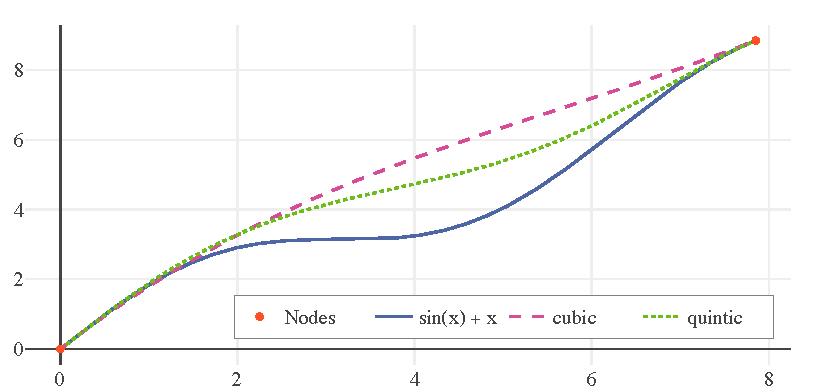
\includegraphics[width=.7\textwidth]{cubic-quintic-sin}
%%   \caption{Depicted above are the monotone cubic and quintic spline interpolants of the function $\sin(x) + x$ over the points $[0, (5/2) \pi]$.  Notice that the maximum error of the cubic interpolant is larger, because it only captures first derivative information at the points. The quintic interpolant captures both first and second derivative information at the points.}
%% \end{figure}

%% \begin{figure}
%%   \centering
%%   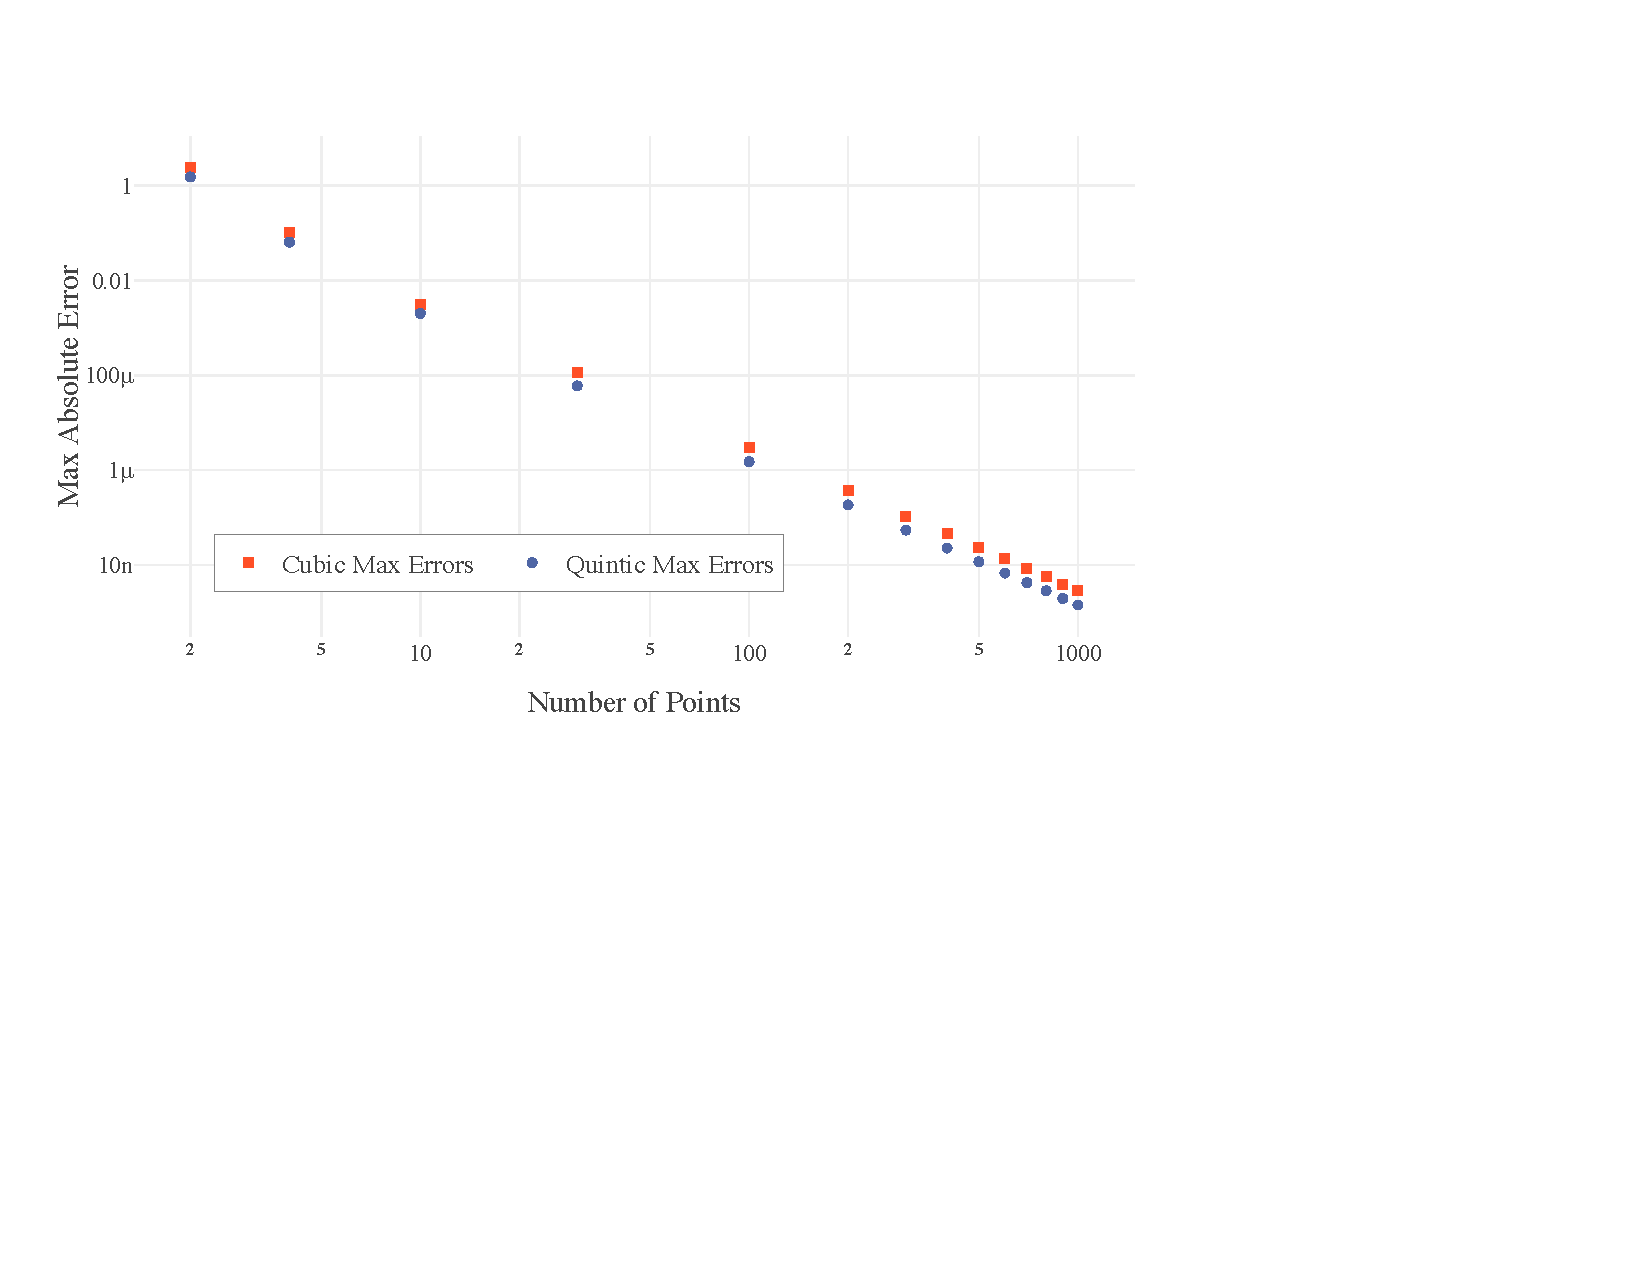
\includegraphics[width=.7\textwidth]{experiment_1_errors}
%%   \caption{The error in the quintic and cubic approximations of $\sin(x) + x$ with increasing number of points. Both axes are log scaled, where $\mu$ means $\times 10^{-6}$ and n means $\times 10^{-9}$ on the vertical axis. The quintic approximation generally provides an approximation with about half of the maximum error of the cubic approximation, while the relative gap between grows with increasing number of points. In order to achieve the same absolute error the quintic spline requires ten fewer points at max error $10^{-4}$, thirty fewer points at max error $10^{-6}$, and $300$ fewer points at max error $10^{-8}$.}
%% \end{figure}

\heading{3.2 \enspace Random Number Generation}

Consider the cumulative distribution function (CDF) defined by a mixture of three Gaussian distributions and visualized in Figure \ref{fig:experiment_2_distribution}. The distributions have weights $(.3, .6, .1)$, means $(.2, .45, .85)$ and standard deviations $(.05, .08, .03)$. $200$ random samples are generated from this distribution with both cubic and quintic approximations from four points, and over $100$ trials the resulting spread of empirical distribution functions (EDFs) are visualized in Figure \ref{fig:experiment_2_results}.

While an increased number of points could be used to decrease the error in either approximation, the purpose of this experiment is to demonstrate the effect approximation error has on random number generation. The errors in the CDFs are magnified by the variance involved in randomly sampling from a distribution. As a result, while the cubic and quintic spline approximations have similar maximum error, the cubic distribution is significantly distorted around the first and second modes.

%% \begin{figure}
%%   \centering
%%   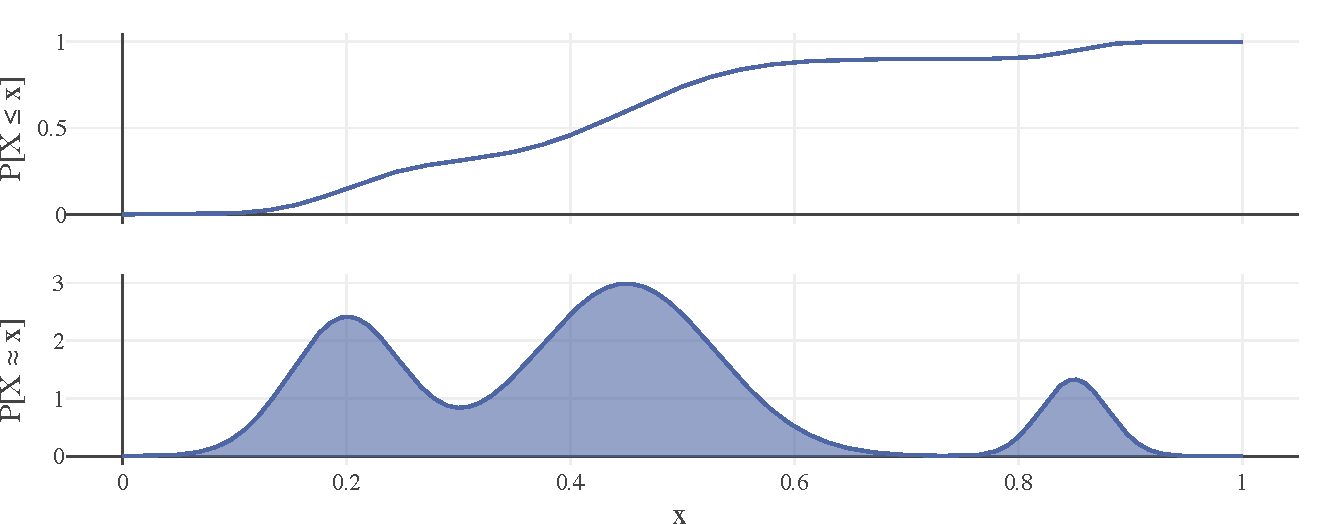
\includegraphics[width=.8\textwidth]{experiment_2_distribution}
%%   \caption{The cumulative distribution function (top) and probability density function (bottom) for the Gaussian mixture distribution in Experiment 2. The distributions have weights $(.3, .6, .1)$, means $(.2, .45, .85)$ and standard deviations $(.05, .08, .03)$. Random samples are generated from this mixture distribution by evaluating the inverse of the CDF at random numbers uniformly distributed in the range $[0,1]$.}
%% \end{figure}

%% \begin{figure}
%%   \centering
%%   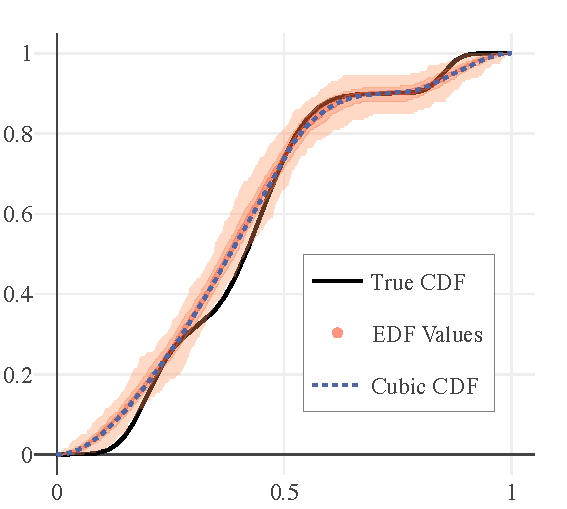
\includegraphics[width=.4\textwidth]{experiment_2_cubic_dist}
%%   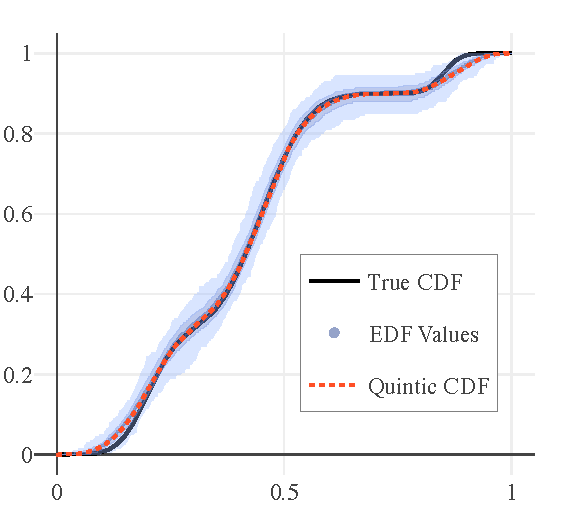
\includegraphics[width=.4\textwidth]{experiment_2_quintic_dist}
%%   \caption{Both cubic and quintic splines are used to approximate the CDF of a Gaussian mixture distribution with three components. Four CDF points are used to build the approximation, $200$ random samples are generated with the approximate CDFs over $100$ trials. The resulting cloud of empirical distribution function (EDF) values is seen above. The maximum approximation error in the CDFs are similar, $.08$ for the cubic and $.05$ for the quintic. However, the maximum EDF differences observed are doubled by the variance of random samples, $.15$ for the cubic and $.1$ for the quintic.}
%% \end{figure}

%% - generate large sets of random monotone data, show Table of number
%%   of metrics growing with increasing number of points

%% - show visual of the \textit{error} 

\heading{3.3 \enspace Random Monotone Data}

This experiment studies the number of times the algorithms {\tt is\_monotone} and {\tt make\_monotone} are executed for increasingly large sequences of random monotone data. The minimum, median, and maximum number of times that Algorithms \ref{alg:check-monotone} and \ref{alg:make-monotone} are executed is recorded, as well as the number of steps taken in all calls to {\tt binary\_search}. The number of calls and steps grows linearly with $n$ as expected, requiring roughly one call to {\tt make\_monotone} and $20$ binary search steps to create a monotone piece. Some (less common) problems require an average of three calls to {\tt make\_monotone} per interval.

%% \begin{table}
%%   \centering
%%   \caption{The minimum, median, and maximum number of checks, fixes, and binary search steps required in the execution of {\tt make\_spline} for increasing size sequences, $n$, over $100$ randomly generated sets of monotone data. Notice the maximum for each counter is often significantly greater than the minimum and median, because the distribution of each counter is skewed right.}

%%   \begin{tabular}{c|c c c|c c c|c c c}
%%     \hline
%%     \multirow{2}{*}{$n$}
%%       & \multicolumn{3}{c|}{Checks} & \multicolumn{3}{c}{Fixes} & \multicolumn{3}{|c}{Search Steps} \\
%%       & min & median & max & min & median & max & min & median & max \\
%%     \hline
%%     5 & 4 & 6 & 274 & 0 & 1 & 154 & 3 & 31 & 2006\\
%%     25 & 28 & 47 & 378 & 2 & 14 & 225 & 80 & 348 & 3742\\
%%     50 & 61 & 124 & 484 & 6 & 40 & 238 & 217 & 851 & 4445\\
%%     75 & 102 & 216 & 842 & 14 & 74 & 411 & 463 & 1491 & 6333\\
%%     100 & 142 & 306 & 776 & 21 & 107 & 380 & 629 & 2140 & 7414\\
%%     \hline
%%   \end{tabular}
%% \end{table}

\heading{4. DISCUSSION}

The monotone quintic spline interpolant provides a distinct increase in accuracy over the monotone cubic variant. The computational complexity of this algorithm is identical to the existing cubic method and the cost of evaluating the spline after construction is unchanged. While the number of computations required per interval has increased, the number of points required to achieve the same level of accuracy has decreased. In the present state, the algorithm for enforcing monotonicity on a spline is not as trivially parallel as the cubic algorithm, however it can still be parallelized. The checks for monotonicity across all intervals are independent and the monotonicity adjustments could be computed independently and intelligently merged with minor changes to the serial algorithm.

Acknowledging that the algorithm for constructing a monotone quintic spline interpolant is slightly more expensive than the cubic case, gains in accuracy or decreased necessary number of points are often worth the computational effort. In practice the costs of spline interpolation are often dominated by evaluation rather than construction, and the increased accuracy is afforded for a negligible increase in computational cost.

\heading{5. CONCLUSION AND FUTURE WORK}

This paper proposes and tests an algorithm for constructing monotone quintic spline interpolants. Experiments demonstrate an improvement in approximation accuracy over monotone cubic spline interpolants, as expected based on theory. There are still open avenues of research going forward, such as an alternative sufficient condition for enforcing monotonicity or increased order monotone approximations. If the monotonicity conditions can be generalized to any order or made linear, the search for a monotone interpolating spline could potentially be formulated as a convex optimization problem. Finally, this work could be used to improve cumulative distribution function (CDF) estimates as well as predictive models that use CDFs.


\heading{Acknowledgments}
This work was supported by the National Science Foundation Grants CNS-1565314 and CNS-1838271.


\heading{\hlvVIII BIBLIOGRAPHY} %% {\let\caps=\capsVIII \let\sl=\slVIII
%% \def\ys{\hskip 1em minus .5em}\let\rm=\rmeight \rmVIII
%% \newcount\refnum \refnum=0 \parskip=2pt plus 2pt minus 2pt
%% \frenchspacing

\bibliography{mqsi20}
\bibliographystyle{plain}

\vfill\eject\end




%% %\refj is for regular journal articles
%% \def\refj#1#2#3#4#5{\noindent\hangindent=10pt\hangafter=1
%% %\global\advance\refnum by 1[\number\refnum]
%% {\caps #1}\ys #2.\ys {\rm #3}. {\sl #4}, #5.\par}

%% %\refb is for books
%% \def\refb#1#2#3#4{\noindent\hangindent=10pt\hangafter=1
%% %\global\advance\refnum by 1[\number\refnum]
%% {\caps #1}\ys #2.\ys{\sl #3}. {\rm #4}.\par}

%% %\refp is for private communication
%% \def\refp#1#2#3{\noindent\hangindent=10pt\hangafter=1
%% %\global\advance\refnum by 1[\number\refnum]
%% {\caps #1}\ys #2.\ys{\rm #3}.\par}

%% %\reft is for tech. reports, theses, and conferences
%% \def\reft#1#2#3#4{\noindent\hangindent=10pt\hangafter=1
%% %\global\advance\refnum by 1[\number\refnum]
%% {\caps #1}\ys #2.\ys{\rm #3}. {\rm #4}.\par}

%% %%%%% top of refs
%% \reft{Amos, B. D., Easterling, D. R., Watson, L. T., Thacker, W. I.,
%% Castle, B. S., Trosset, M. W.}{2014}{Algorithm XXX: QNSTOP: Quasi-Newton
%% algorithm for stochastic optimization}{Technical Report 2014-07,
%% Virginia Polytechnic Institute and State University, Blacksburg, VA}

%% \refb{Anderson, E., Bai, Z., Bischof, C., Blackford, S., Demmel, J.,
%% Dongarra, J., Du Croz, J., Greenbaum, A., Hammarling, S., McKenney, A.,
%% and Sorensen, D.}{1999}{LAPACK Users' Guide Third Edition}
%% {SIAM, Philidelphia, PA}

%% \refb{Aurenhammer, F., Klein, R., and Lee, D. T.}{2013}
%% {Voronoi diagrams and Delaunay triangulations}
%% {World Scientific Publishing Co., Hackensack, NJ}

%% \refj{Barber, C. B., Dobkin, D. P., and Huhdanpaa, H.}{1996}
%% {The Quickhull algorithm for convex hulls}{ACM Trans. Math.
%% Softw. 22}{469--483}

%% \reft{Boissonnat, J.-D., Devillers, O., and Hornus, S.}{2009}
%% {Incremental construction of the Delaunay triangulation and the
%% Delaunay graph in medium dimension}{In {\sl Proc. Twenty-fifth Annual Symp.
%% on Computational Geometry}, ACM, New York, NY, 208--216}

%% \refj{Bowyer, A.}{1981}{Computing Dirichlet tessellations}
%% {The Computer Journal 24}{162--166}

%% \refj{Cameron, K. W., Anwar, A., Cheng, Y., Xu, L., Li, B., Ananth, U.,
%% Bernard, J., Jearls, C., Lux, T., Hong, Y., Watson, L. T.,
%% and Butt, A. R.}{2019}{MOANA: modeling and analyzing I/O variability
%% in parallel system experimental design}
%% {IEEE Trans. Parallel Distrib. Systems}{to appear}

%% \reft{Chang, T. H., Watson, L. T., Lux, T. C. H., Bernard, J., Li, B.,
%% Xu, L., Back, G., Butt, A. R., Cameron, K. W., and Hong, Y.}{2018a}
%% {Predicting system performance by interpolation using a high-dimensional
%% Delaunay triangulation} {In {\sl Proc. 2018 Spring Simulation Multiconference,
%% 26th High Performance Computing Symp.}, Soc. for Modelling and Simulation
%% Internat., Vista, CA, Article No. 2}

%% \reft{Chang, T. H., Watson, L. T., Lux, T. C. H., Li, B., Xu, L., 
%% Butt, A. R., Cameron, K. W., and Hong, Y.}{2018b}{A polynomial time
%% algorithm for multivariate interpolation in arbitrary dimension via
%% the Delaunay triangulation} {In {\sl Proc. ACM 2018 Southeast Conference
%% (ACMSE '18)}, ACM, New York, NY, Article No. 12}

%% \refb{Cheney, E. W. and Light, W. A.}{2009}
%% {A Course in Approximation Theory}{American Mathematical Soc., 
%% Providence, RI}

%% \refb{Cheng, S. W., Dey, T. K., and Shewchuk, J.}{2012}
%% {Delaunay Mesh Generation}{Computer and Information Science
%% Series, CRC Press, New York, NY}

%% \refj{Cignoni, P., Montani, C., and Scopigno, R.}{1998}
%% {DeWall: A fast divide \& conquer Delaunay triangulation algorithm in $E^d$}
%% {Computer-Aided Design 30}{333--341}

%% \refb{de Berg, M., Cheong, O., van Kreveld, M., and Overmars, M.}{2008}
%% {Computational Geometry: Algorithms and Applications}{Springer-Verlag,
%% Berlin, Germany}

%% \refj{Devillers, O., Pion, S., and Teillaud, M.}{2002}
%% {Walking in a triangulation}{Internat. Journal of Foundations of
%% Computer Science 13}{181--199}

%% \reft{Edelsbrunner, H.}{1989}{An acyclicity theorem for cell complexes in
%% d dimensions} {In {\sl Proc. Fifth Annual Symp. on Computational Geometry}, 
%% ACM, New York, 145--151}

%% \refj{Hanson, R. J. and Haskell, K. H.}{1982}
%% {Algorithm 587: Two algorithms for the linearly constrained least
%% squares problem}{ACM Trans. Math. Softw. 8}{323--333}

%% \refj{Klee, V.}{1980}{On the complexity of d-dimensional Voronoi diagrams}
%% {Archiv der Mathematik 34}{75--80}

%% \reft{Lux, T. C. H., Watson, L. T., Chang, T. H., Bernard, J., Li, B.,
%% Xu, L., Back, G., Butt, A. R., Cameron, K. W., and Hong, Y.}{2018}
%% {Predictive modeling of I/O characteristics in high performance computing
%% systems}{In {\sl Proc. 2018 Spring Simulation Multiconference, 26th High 
%% Performance Computing Symp.}, Soc. for Modelling and Simulation Internat.,
%% Vista, CA, Article No. 8}

%% \refj{M{\"u}cke, E. P., Saias, I., and Zhu, B.}{1999}
%% {Fast randomized point location without preprocessing in two- and 
%% three-dimensional Delaunay triangulations}
%% {Computational Geometry 12}{63--83}

%% \refj{Omohundro, S. M.}{1990}{Geometric learning algorithms}
%% {Physica D: Nonlinear Phenomena 42}{307--321}

%% \reft{OpenMP Architecture Review Board (ARB)}{2015}
%% {OpenMP Application Programming Interface (version 4.5)}
%% {OpenMP}

%% \refj{Rajan, V. T.}{1994}
%% {Optimality of the Delaunay triangulation in $R^d$}
%% {Discrete \& Computational Geometry 12}{189--202}

%% \refj{Schaap, W. E. and van de Weygaert, R.}{2000}
%% {Continuous fields and discrete samples: reconstruction through
%% Delaunay tessellations}{Astronomy and Astrophysics 363}{L29--L32}

%% \refj{Su, P. and Drysdale, R. L. S.}{1997}
%% {A comparison of sequential Delaunay triangulation algorithms}
%% {Computational Geometry 7}{361--385}

%% \refj{Watson, D. F.}{1981}{Computing the n-dimensional Delaunay tessellation
%% with application to Voronoi polytopes}
%% {The Computer Journal 24}{167--172}

%% }\vfill\eject\end
%% %%%%% bottom

